\section{Lower Bounds for the Extension Complexity}
% todo: Think about multi-dimensional proof

In this section we provide yet another proof for $pc(n) \in \Omega(n^{1/2})$.

After the proof is done, we will explain the key concepts of the applied theorem and show how to apply it in general.

The central piece of the proof is Theorem~1 from \cite{averkov2016maximum}, which we adopt for the case of linear extended formulations (the original also allowed semidefinite ones).

We define $\norm{\cdot}$ to be the Euclidean norm and $\B^d := \{ x \in \R^d \mid \norm{x} \leq 1 \}$ to be the $d$-dimensional unit ball.



\subsection{Introducing the Applied Theorem}

Frist we have to define the \textit{Hausdorff distance} of two non-empty compact sets $X,Y \subseteq \R^d$, which can be thought of "the longest distance you can be forced to travel from a point in one of the two sets to the other set". See Figure~\ref{fig:hausdorff} for an example.

\begin{figure}[h]
  \centering
  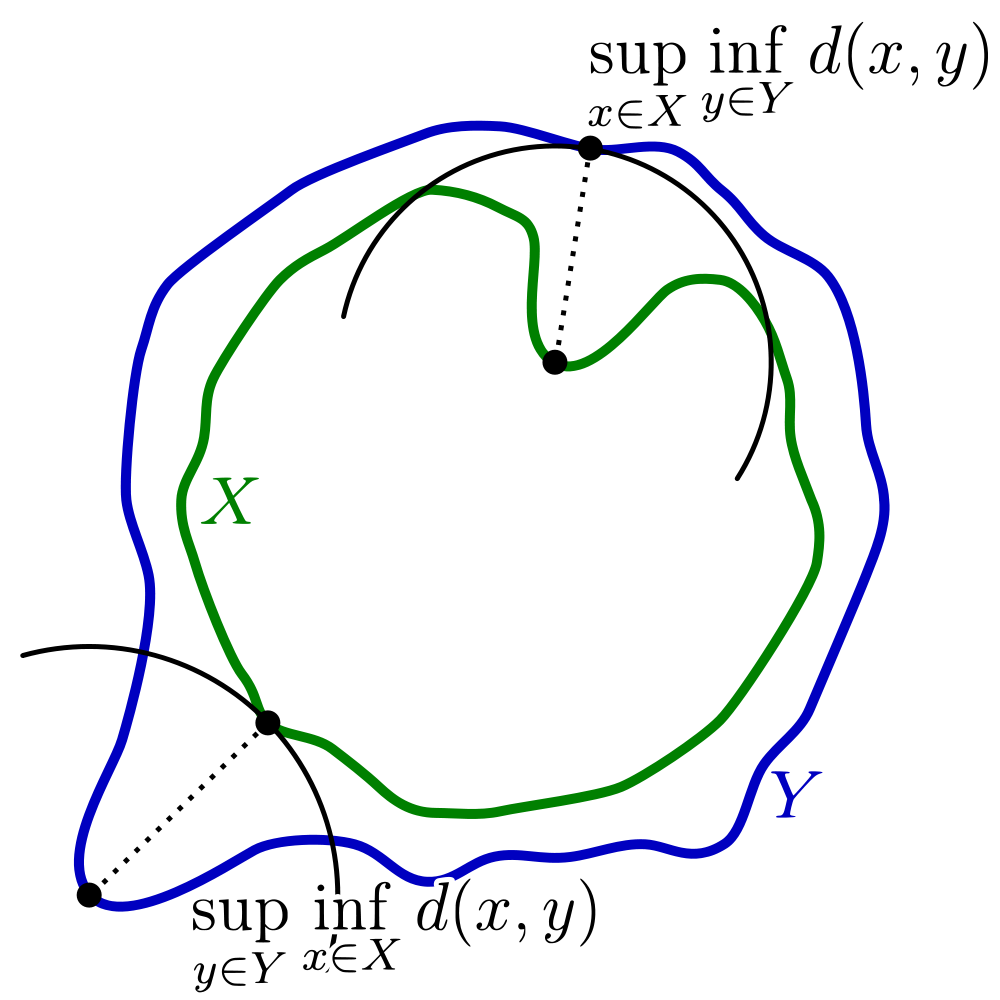
\includegraphics[height=55mm]{assets/Hausdorff_distance.png}
  \caption{Hausdorff distance example \cite{rocchini2007hausdorff}}
  \label{fig:hausdorff}
\end{figure}

\begin{definition}[Hausdorff distance]
  The \textit{Hausdorff distance} with respect to the Euclidean norm is defined by $$ \dist_H(X,Y) := \max \left\{ \adjustlimits \sup_{x \in X} \inf_{y \in Y} \norm{x-y}, \adjustlimits \sup_{y \in Y} \inf_{x \in X} \norm{x-y} \right\} .$$
\end{definition}

\begin{theorem}[{\cite[Theorem 1]{averkov2016maximum}}, adopted]\label{theorem:family}
  Let $\P$ be a family of polytopes in $\R^d$ of dimensions at least one with $2 \leq \abs{\P} < \infty $ such that each $P \in \P$ has an extended formulation of size $m$.
  Let $\rho > 0$ and $\Delta > 0$ be such that each $P \in \P$ is contained in the ball $\rho \B^d$ and, 
  for every two distinct polytopes $P \in \P$ and $P' \in \P$, one has $\dist_H(P, P') \geq \Delta$. 
  Then $$m^2 \geq \frac{\log_2 \abs{\P}}{8d \left(1 + \log_2 (2\rho/\Delta) + \log_2\log_2 \abs{\P} \right)} =: B.$$
  In particular, we have $$\max \{\xc(P) \mid P \in \P\}  \geq \sqrt{B} .$$
\end{theorem}



\subsection{Proof of Lower Bound}

\begin{corollary}\label{corollary:lower-bound}
  $pc(n) \in \Omega(\sqrt{n})$
\end{corollary}
\begin{proof}
  To apply \ref{theorem:family} we have to pick a familiy of polytopes $\P$. Then we have to determine $\rho$ and $\Delta$ and bound $\log_2 \abs{\P}$ from below and $\log_2 \log_2 \abs{\P}$ from above.

  So we choose $n^2$ fixed points evenly on the unit circle (so they would form a regular polygon). Let $\P_n$ be the familiy of polygons, where each polygon has $n$ vertices chosen from the $n^2$ points on the unit circle.

  Then $\rho = 1$, since all polygons are contained in the unit circle.

  For two distinct polygons $P, P' \in \P_n$ one of them has a vertex $v$, which the other one does not have. W.l.o.g $v \notin P, v \in P'$. So $\dist_H(P,P') \geq \inf_{p \in P} \norm{v-p} \geq d_{min}$ (see Figure~\ref{fig:distance} for the definition of $d_{min}$).

  \begin{figure}[h]
    \centering
    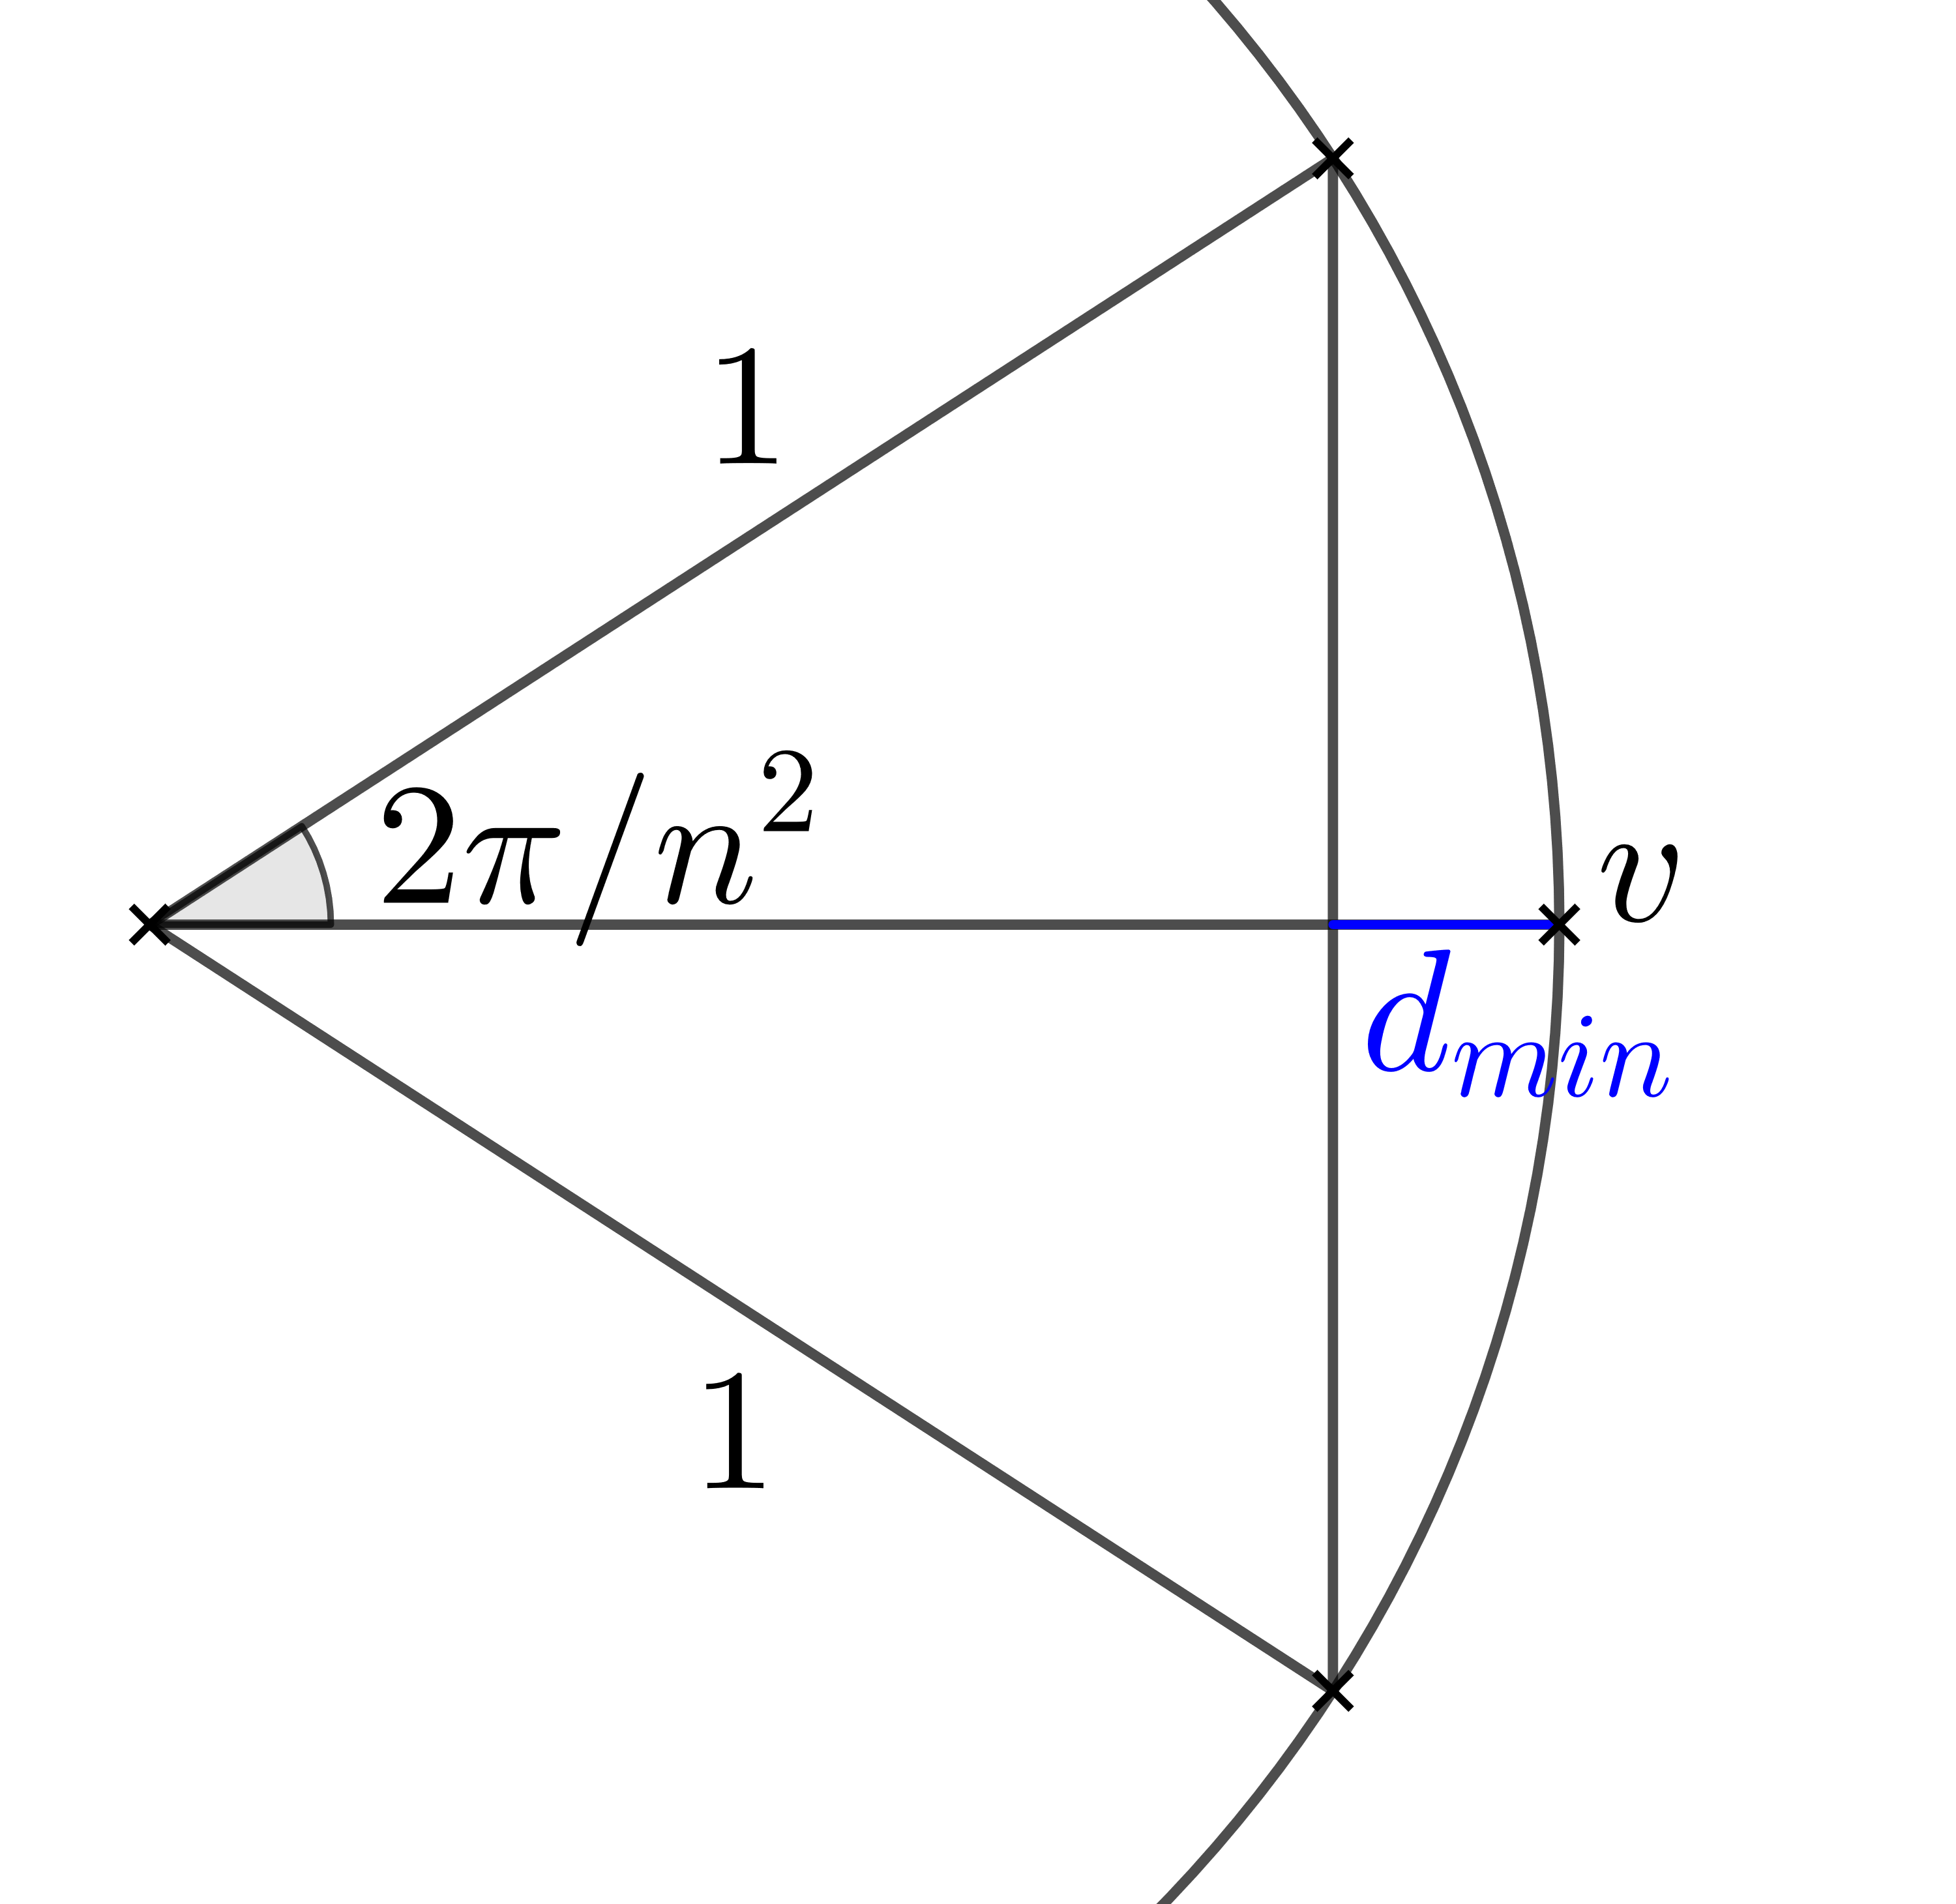
\includegraphics[height=55mm]{assets/Minimal_Hausdorff_distance.png}
    \caption{Definition of $d_{min}$}
    \label{fig:distance}
  \end{figure}

  \begin{align*}
    1 - d_{min} &= \cos\left( \frac{2 \pi}{n^2} \right)\\
    d_{min} &\geq 1 - \left(1 - \frac{\left(\frac{2 \pi}{n^2}\right)^2}{2} \right) = 2 \frac{\pi^2}{n^4} =: \Delta
  \end{align*}

  For the estimate we used $\cos(x) \leq 1 - \frac{x^2}{2!}$, which arises from the power series for cosine.

  Since each polygon in $\P_n$ is defined by $n$ points, chosen from a set of $n^2$ points, $\abs{\P_n} = \binom{n^2}{n}$. Therefore $n^n = \left( \frac{n^2}{n} \right)^n \leq \abs{\P_n} \leq \left( n^2 \right)^n = n^{2n}$. $\log_2 \abs{\P_n} \geq n \log_2 n$ and $\log_2 \log_2 \abs{\P_n} \leq \log_2 (2n \log_2 n) = 1 + \log_2 n + \log_2 \log_2 n$.

  Now we can calculate $B$ from Theorem~\ref{theorem:family}:
  \begin{align*}
    B &= \frac{\log_2 \abs{\P_n}}{8d \left(1 + \log_2 (2\rho/\Delta) + \log_2\log_2 \abs{\P_n} \right)}\\
    &\geq \frac{n \log_2 n}{16 \left(1 + \log_2 (n^4 / \pi^2) + 1 + \log_2 n + \log_2 \log_2 n \right)}\\
    &= \frac{n \log_2 n}{16 \left(2 - 2 \log_2 \pi + 5 \log_2 n + \log_2 \log_2 n \right)}\\
    &\geq \frac{n}{16*6}
  \end{align*}

  For the last inequality we used $2 - 2 \log_2 \pi \leq 0$ and $\frac{5 \log_2 n + \log_2 \log_2 n}{\log_2 n} \leq 6$ for $n \geq 1$.

  Therefore we can conclude $$\pc(n) \geq \max \{\xc(P) \mid P \in \P_n\} \stackrel{\text{(Th. \ref{theorem:family})}}{\geq} \sqrt{B} \geq \frac{1}{12} \sqrt{n} .$$
\end{proof}



\subsection{Key Idea of the Used Theorem~\ref{theorem:family}}

The central idea of \ref{theorem:family} is to encode the extended formulations. Then one counts how many extended formulations fit into the containing volume, since those formulations are seperated themselves.

Here is a short outline of the proof:
\begin{enumerate}
  \item Each extended formulation can be normalized, i.e. $P = \varphi(Q) + t$ with $Q = \{ x \mid Ax \leq \mathbbm{1} \}$, $\mathbb{B}^n \subseteq Q \subseteq n\mathbb{B}^n$ and $\varphi$ being linear.
  \item Each polytope $P_i \in \P$ ($P_i = \varphi_i(Q_i) + t_i$, $Q_i = \{ x \in \R^{n_i} \mid A_ix \leq \mathbbm{1} \}$) is encoded trough $P_i \mapsto (A_i, \varphi_i, t_i)$.\\
  From now on everything takes place in the encoding vector spaces $\mathcal{V^n}$, where $n$ is the dimension of the extended formulation.
  \item The encodings are partitioned into sets $W_i$ by the dimension of $Q_i$.
  \item The distance between two encodings $w, w' \in W_i$ can be bounded by $\norm{w - w'} \geq \Delta$.
  \item The overall space required can be bounded by $\norm{w} \leq 3\rho n^2 \forall w \in W_i$.
  \item One creates small balls around each encoding with radius $\Delta/2$ and a ball containing all small balls with radius $3\rho n^2 + \Delta/2$ around the origin.
  \item By comparing volumes, one can bound $\abs{W_i}$ from above depending on $\rho$, $\Delta$, $m$ and~$d$.
  \item These bounds are joined together for all $W_i$ and solved for $m$.
\end{enumerate}

The lower bounding of $\xc$ ($\max \{\xc(P) \mid P \in \P\}  \geq \sqrt{B}$) is achieved by inverting the implication: 
$$ \left( \left( \forall P\in\P: \xc(P) \leq m \right) \Rightarrow m^2 \geq B \right) \Rightarrow \left( m^2 < B \Rightarrow \left( \exists P\in\P: xc(P) > m \right) \right) $$

This theorem is applied easily like in Corollary~\ref{corollary:lower-bound} by picking a familiy $\P$ and then bounding $\rho$ from above, $\Delta$ from below, $\log_2 \abs{\P}$ from below and $\log_2\log_2 \abs{\P}$ from above. This theorem then provides a lower bound for the largest extension complexity of one polytope $P \in \P$.
